%% Copyright 1998 Pepe Kubon
%%
%% `two.tex' --- 2nd chapter for thes-full.tex, thes-short-tex from
%%               the `csthesis' bundle
%%
%% You are allowed to distribute this file together with all files
%% mentioned in READ.ME.
%%
%% You are not allowed to modify its contents.
%%

%%%%%%%%%%%%%%%%%%%%%%%%%%%%%%%%%%%%%%%%%%%%%%%%%
%
%     Chapter 4  
%
%%%%%%%%%%%%%%%%%%%%%%%%%%%%%%%%%%%%%%%%%%%%%%%%

\chapter{A Pruning-based Method}
\label{ch:pruning}

%To speed up query processing, we are interested in an efficient and effective filtering technique instead of the exact computation of similarity scores for all objects regarding an updated query. 

Computing the exact similarity score for every object against the updated query at every time point is costly.  We derive an upper bound of Jaccard similarity scores in Section~\ref{sec:jac-bound}, and then present a pruning-based method that utilizes the upper bounds in Section~\ref{sec:pruning-method}. In Section~\ref{sec:gen-sim}, we claim that the proposed method can be used as a framework for many other similarity measures including Cosine similarity and Edit similarity. We review the definitions of these similarity measures and then derive the upper bounds that can be computed in constant time. 

\section{A Progressive Upper Bound}
\label{sec:jac-bound}
Let us denote the lengths of an object and the query as $|X|$ and $|Y|$, respectively. Based on the definition of count-based sliding windows, %we define updates of a query as follows.
%
%\begin{definition}
%(Updates of a query). Let us denote $SW$ as a collection of elements in the current sliding window. The current query $q$ is defined as the set of distinct elements in $SW$. Suppose $SW=\{e_1, e_2,..., e_n\}$, the updated sliding window after $u$ time instants is $SW'=\{e_{u+1}, e_{u+2}, ..., e_{|q|}, e_{new_1}, e_{new_2}, ..., e_{new_u}\}$, where $u$ is a positive integer and $u<n$. Similarly, the updated query $q'$ after $u$ time instants is the set of distinct elements in $SW'$.
%\end{definition}
%
%\begin{definition}[Updates of a query] G
given a query $q=\{e_1, e_2,..., e_{|q|}\}$, the updated query after $u$ time instants is $q'=\{e_{u+1}, e_{u+2}, ..., e_{|q|}, e_{new_1}, e_{new_2}, ..., e_{new_u}\}$, where $u$ is a positive integer and $u<|q|$.
%\end{definition}

To compute the upper bound for Jaccard similarity score after $u$ updates, we can use the following property.
%, whose proof is given in Appendix~\ref{proof:progressive-upper-bound}.

\begin{property}[A Progressive Upper Bound for Jaccard Similarity]%\label{ppt:progressive-upper-bound}
Given the weighted Jaccard similarity score $sim_{Jac}(X, Y)$ between two multisets $X$ and $Y$, and without the knowledge of the updated multiset $Y_u'$ after $u$ updates on $Y$, we have
% the upper bound for the weighted Jaccard similarity score after $u$ updates 
$$sim_{Jac}(X, Y_u') \leq \frac{(|X|+|Y|+u)\cdot sim_{Jac}(X, Y)+u}{|X|+|Y|-u\cdot sim_{Jac}(X, Y)-u}.$$
\end{property}

\begin{proof}
By definition, we have $$sim_{Jac}(X, Y) = \frac{\sum_{i=1}^{|\Sigma|} \min\{x_i, y_i\}}{\sum_{i=1}^{|\Sigma|} \max\{x_i, y_i\}}$$ and $\sum_{i=1}^{|\Sigma|} \max\{x_i, y_i\}=|X|+|Y|- \sum_{i=1}^{|\Sigma|} \min\{x_i, y_i\}$. Using the above two equations, we have $$\sum_{i=1}^{|\Sigma|} \min\{x_i, y_i\} =\frac{(|X|+|Y|)\cdot sim_{Jac}(X, Y)}{sim_{Jac}(X, Y)+1}.$$ 
Thus, 
\begin{align*}
& sim_{Jac}(X, Y_u') \\
\leq & \frac{u+\sum_{i=1}^{|\Sigma|} \min\{x_i, y_i\}}{-u+\sum_{i=1}^{|\Sigma|} \max\{x_i, y_i\}} \\
= & \frac{u+\sum_{i=1}^{|\Sigma|} \min\{x_i, y_i\}}{-u+|X|+|Y|-\sum_{i=1}^{|\Sigma|} \min\{x_i, y_i\}} \\
= & \frac{u+\frac{(|X|+|Y|)\cdot sim_{Jac}(X, Y)}{sim_{Jac}(X, Y)+1}}{-u+|X|+|Y|-\frac{(|X|+|Y|)\cdot sim_{Jac}(X, Y)}{sim_{Jac}(X, Y)+1}} \\
= & \frac{(|X|+|Y|+u)\cdot sim_{Jac}(X, Y)+u}{|X|+|Y|-u\cdot sim_{Jac}(X, Y)-u}
\end{align*}
\end{proof}

\begin{example}[Computation of Progressive Upper Bound for Jaccard Similarity] 
Let us consider the same multisets $X$ and $Y$ as in Example~\ref{computeSim}. We have $|X|=5$, $|Y|=6$, and $sim_{Jac}(X, Y) = 0.57$. Suppose $u=1$, the upper bound of the Jaccard similarity after an update is $sim_{Jac\_up}(X, Y_1') = 0.85$.
\end{example}

%\subsection{Static Upper Bound Based on Object Lengths} 
%\begin{property}
%(Upper bound for weighted Jaccard similarity).
%Given two multisets $X$ and $Y$ and without loss of generality, suppose their sizes satisfy $|X|\leq|Y|$, the upper bound for the weighted Jaccard similarity score $sim_{Jac}(X, Y)$ is $\frac{|X|}{|Y|}$. 
%\end{property}

%\begin{proof}
%By Definition~\ref{wjacdef}, 
%$$sim_{Jac}(X, Y)=\frac{\sum_{i=1}^{|\Sigma|} \min\{x_i, y_i\}}{\sum_{i=1}^{|\Sigma|} \max\{x_i, y_i\}}$$
%$$\leq \frac{\min\{\sum_{i=1}^{|\Sigma|} x_i, \sum_{i=1}^{|\Sigma|} y_i\}}{\max\{\sum_{i=1}^{|\Sigma|} x_i, \sum_{i=1}^{|\Sigma|} y_i\}}$$ 
%$$=\frac{\min\{|X|, |Y|\}}{\max\{|X|, |Y|\}}=\frac{|X|}{|Y|}.$$
%\end{proof}

\section{A Pruning-based Algorithm (GP)}
\label{sec:pruning-method}
A brute-force method is to compute the similarity score between the updated query and each object at each time instant, and then sort the scores and get the top-$k$ list. This approach is costly and involves heavy unnecessary computation, since when the query window slides only a small number of positions, e.g., 1 or 2, the changes of the similarity scores are limited. We present a heuristic algorithm that finds the exact top-$k$ objects continuously, as shown in Algorithm~\ref{GPmain}. Table~\ref{Symbols} lists the symbols used in the GP algorithm.

%For clearer presentation of our method, let us assume that the arrival of new element is synchronized with time, \emph{i.e.}, a new element arrives at the stream whenever there is an update in time. 
The query at time $t+1$ shares a large portion of elements (at least $\frac{n-1}{n}$) with the query at time $t$. Thus, if $n$ is large, we do not expect a dramatic change in the top-$k$ list, which means that the probability is low that the transactions with large similarity scores at time $t$ may leave the top-$k$ list at time $t+1$.  Similarly, the probability is also low that the transactions with small similarity scores at time $t$ may enter the top-$k$ list at time $t+1$. 


\begin{table}[tb]
\centering
\caption{Symbols Used in the Pruning-based Algorithms}
%\small
\begin{tabular}{|l|p{11cm}|} \hline
      Symbol & Interpretation \\ \hline
      $T_i$ & the $i^{th}$ object/transaction in a database (DB)\\ \hline
      $m$ & number of objects/transactions \\ \hline
      $q_t$ & the query at time $t$ that consists of the elements in the sliding window at time $t$ \\ \hline
      $n$ & size of the sliding window, \emph{i.e.}, query length\\ \hline
      $sim(T_i,T_j)$ & the exact similarity of two objects, $T_i$ and $T_j$\\ \hline
      $sim(T_i, T_j)_{up}$ & the upper bound of similarity score of two objects, $T_i$ and $T_j$\\ \hline
      % $sim(T_i,T_j)_{lo}$ & the lower bound of similarity score of two objects, $T_i$ and $T_j$\\ \hline
      $\Delta sim(T_i)_{+}$ & the maximum increase in similarity score regarding the next query\\ \hline 
      % $\Delta sim(T_i)_{-}$ & the maximum decrease in similarity score regarding the next query\\ \hline 
      % $dis(T_i,T_j)$ & the exact distance of two objects, $T_i$ and $T_j$\\ \hline
      $k$ & number of objects in the result \\ \hline
      $topk_{t}$ & the set of $k$ objects that are most similar to the query at time $t$\\ \hline
      $k^{th}best$ & the $k^{th}$ best result in the current result set\\ \hline
      $u_i$ & the estimated least number of updates needed for object $T_i$ to enter $topk$ \\ \hline
\end{tabular}
  \label{Symbols}
\end{table}

\begin{algorithm2e}[htb]
\SetAlgoLined%\small
 \SetKwInput{Input}{Input}
 \SetKwInput{Output}{Output}
 \caption{A General Pruning Algorithm (GP)}
 \label{GPmain}
 \Input{$q_t$; $m$ objects; $topk_{t-1}$; similarity score regarding $q_{t-1}$ or its upper bound for each object; $u_i$ for each object.}
 \Output{$topk_{t}$}

 Compute exact similarity scores for objects in $topk_{t-1}$ regarding $q_t$ and initialize $topk_t$ with the scores\;
 \ForEach{$T_i$ in DB but not in $topk_{t-1}$}{
  \eIf{$u_i \leq 1$}{
   Compute $sim(T_i, q_t)$\; 
   $u_i \gets$ Null\;
   \If{$sim(T_i, q_t) > k^{th}best$}{
   Update $topk_t$\;}
   }
   {
   \eIf{$sim(T_i, q_t)_{up} \leq k^{th}best$}
   {$u_i \gets u_i - 1$\;}
   {
   Compute $sim(T_i, q_t)$\; 
   $u_i \gets$ Null\; 
   \If {$sim(T_i, q_t) > k^{th}best$}
   {Update $topk_t$\;}
   }
   }
   \ForEach{$T_i$ in DB}{
   \If{$u_i =$ Null} 
   {$est\_bound\left(sim(T_i, q_t), k^{th}best \right)$\;}
   }
 }
\end{algorithm2e}

\begin{algorithm2e}[htb]
 \SetAlgoLined%\small
 \SetKwInput{Input}{Input}
 \SetKwInput{Output}{Output}
  \SetKwInput{Prototype}{Function}
 \caption{Update $u_i$ and Similarity Bounds after Re-computation of Similarity Scores}
\label{GPsub}
\Prototype{$est\_bound(sim(T_i, q_t), k^{th}best)$}
 \Input{$sim(T_i, q_t)$; $k^{th}best$ in $topk_t$; }
 \Output{$u_i; sim(T_i, q_t)_{up}$.}
 
  \eIf{$sim(T_i, q_t) < k^{th}best$}{
  Compute $\Delta sim(T_i)_{+}$\;
  $u_i \gets \lceil \frac{k^{th}best-sim(T_i, q_t)}{\Delta sim(T_i)_{+}}\rceil$\;
  $sim(T_i, q_t)_{up} \gets $ tight upper bound after $u_i$ updates\;  
  }
  {$u_i \gets 0$\; $sim(T_i, q_t)_{up} \gets sim(T_i, q_t)$\;}
  Output $u_i$, $sim(T_i, q_t)_{up}$\;
 \end{algorithm2e}
 
We can divide the objects into three groups according to their current similarity scores. In the first group, the similarity scores associated with the objects are large enough so that in the next several updates, the objects will not leave the top-$k$ list. In the second group, the similarity scores are small enough so that the objects will not enter the top-$k$ list in the next several updates. The last group consists of those ``boundary'' objects, which have relatively high potential of either leaving or entering the top-$k$ list. 

For the objects in the first two groups, there is no need to compute the exact scores in the next time instant. We only need to compute their upper or lower bounds at the next update. To further reduce computation cost, we do not compute bounds in each update. Instead, we estimate $u_i$, the least number of updates needed for an object to enter or leave the top-$k$ list and compute the bounds after the estimated number of updates. The computation details are described in a subroutine shown in Algorithm~\ref{GPsub}. If the estimated value $u_i$ is no more than one, we regard object $T_i$ as a ``boundary'' object in this update. In the other case where $u_i$ is greater than one, we compare the precomputed upper bound with the minimum score in the current top-$k$ list. If the upper bound is smaller than the minimum score, we do nothing but decrement $u_i$ by one. Otherwise, this object is identified as ``boundary''.

For a ``boundary'' object that has a good chance of entering the list, we compute the exact similarity score. If the score is greater than the minimum score in the top-$k$ list, this object enters the list and the object with the smallest score in the list leaves. After all the objects are processed once, for each ``boundary'' object identified at the current time instant, we re-estimate the least number of updates needed for an object and compute the corresponding upper bound. 
%This method is illustrated formally in Algorithm~\ref{GPmain}. 
In our implementation, we maintain a min-heap with $k$ elements that stores the top-$k$ objects for efficient updates.

%The last thing to mention is about the exactness of this method. 
Finally, we discuss the exactness of this method. To ensure that our method can find the exact top-$k$ objects in each update, we first compute the exact similarity scores between the updated query and each object in the top-$k$ result of the previous query. The top-$k$ list is updated accordingly. The other objects are then processed one by one. The top-$k$ list always consists of the $k$ objects with the largest similarity scores among the objects that have been processed so far. Since the minimum score in the top-$k$ list does not decrease during this process, if the score of an object is smaller than the minimum score in the top-$k$ list when it is processed, it must be smaller than the minimum score of the exact top-$k$ list. Therefore, the algorithm always returns the exact top-$k$ result. 

\section{Generalization to Other Similarity Measures}
\label{sec:gen-sim}
% add applications of edit distance and cosine similarity, reason for extending the method
String similarity search is a fundamental operation in many applications such as data cleaning, information retrieval, and bioinformatics~\cite{DLFL13}. Edit distance is often used to measure the dissimilarity of strings.

Cosine similarity has been widely used for comparing the similarity among documents. A document can be represented by a vector where each component is the frequency of a particular word in the document. This type of term-frequency vector is used in applications including information retrieval, text document clustering, biological taxonomy, and gene feature mapping~\cite{HkP11}.        

To efficiently apply the framework proposed in Section~\ref{sec:pruning-method} to other similarity measures, we need to derive efficient and effective bounds for future updates based on current similarity/distance and its related functions. In this section, we show that the progressive bounds for edit distance, edit similarity, and cosine similarity can be computed in constant time.    

 
\subsection{Edit Distance and Edit Similarity}

\begin{definition}[Edit Distance and Edit Similarity]\label{def:edit-gen}
Given two strings $X$ and $Y$ of length $m$ and $n$ respectively, the edit distance $dis_{ed}(X, Y)$ is the minimum cost required to convert $X$ to $Y$. Typically, we consider three edit operations, namely, insertion, deletion and substitution. The costs of three edit operations, denoted by $\delta_i$, $\delta_d$ and $\delta_s$, are non-negative and can be different. The edit similarity is defined as $$sim_{ed}(X, Y) = 1 - \frac{dis_{ed}(X, Y)}{\max\{\delta_i, \delta_d, \delta_s\}\cdot \max\{|X|, |Y|\}}.$$
\end{definition}

\begin{example}[Computation of Edit Similarity]\label{example:comp-edit}
Suppose the costs of insertion, deletion and substitution are 2, 1, and 3, respectively. $X = ababb$ and $Y = bbabac$ are two strings that consist of symbols in alphabet $\Sigma=\{a, b, c\}$. The edit distance table is shown in Table~\ref{edit01}. From the table, we have $dis_{ed}(X, Y) = 8$. Thus, the edit similarity score between $X$ and $Y$ is $sim_{ed}(X, Y) = 1- \frac{8}{3\times 6} = 0.44$.
\end{example}

\begin{table}[tb]
\caption{Edit distance tables for Example~\ref{example:comp-edit} and Example~\ref{example:bound-ed}}
\label{ed-comp}
\centering
\subfigure[$\delta_i=2, \delta_d=1, \delta_s=3$]{% a
\begin{tabular}{|c||c|c|c|c|c|c|c|} \hline
      &$\epsilon$&b&b&a&b&a&c\\ \hline \hline
      $\epsilon$&0&2&4&6&8&10&12 \\ \hline
      a&1&3&5&4&6&8&10 \\ \hline
      b&2&1&3&5&4&6&8 \\ \hline
      a&3&2&4&3&5&4&6 \\ \hline
      b&4&3&2&4&3&5&7 \\ \hline
      b&5&4&3&5&4&6&8 \\ \hline
    \end{tabular}
    
    \label{edit01}
}
\quad
\subfigure[$\delta_i=\delta_d=\delta_s=1$]{% b
\begin{tabular}{|c||c|c|c|c|c|c|c|} \hline
      &$\epsilon$&b&b&a&b&a&c\\ \hline \hline
      $\epsilon$&0&1&2&3&4&5&6 \\ \hline
      a&1&1&2&2&3&4&5 \\ \hline
      b&2&1&1&2&2&3&4\\ \hline
      a&3&2&2&1&2&2&3\\ \hline
      b&4&3&2&2&1&2&3\\ \hline
      b&5&4&3&3&2&2&3\\ \hline
    \end{tabular}
    
    \label{edit02}
}

\end{table}


Since edit similarity is a function/transformation of edit distance, we first compute the upper and lower bounds for edit distance. We show in Property~\ref{ppt:tri-ineq-ed} that edit distance satisfies triangle inequality. Thus, we can derive the upper and lower bounds of edit distance using triangle inequality as shown in Property~\ref{ppt:bound-ed}. Property~\ref{ppt:bound-es} shows the bounds for edit similarity. 

\begin{property}[Triangle Inequality of Edit Distance]\label{ppt:tri-ineq-ed}
Given any three strings $X$, $Y$, and $Z$, the edit distance between $X$ and $Y$ satisfies the following triangle inequality. 
$$dis_{ed}(X,Y) \leq dis_{ed}(X,Z)+dis_{ed}(Z,Y).$$
\end{property}

\begin{proof}
If we want to transform string $X$ into string $Y$, we can first transform $X$ into another arbitrary string $Z$ and then transform $Z$ into $Y$. This kind of two-step edit operation may not have the cheapest cost. Thus, we have $dis_{ed}(X,Y) \leq dis_{ed}(X,Z)+dis_{ed}(Z,Y).$ That is, edit distance satisfies triangle inequality. As shown in Figure~\ref{triIneqa}, we can think of $XY$ to be the shortest path between $X$ and $Y$. An alternative path that consists of two edges $XZ$ and $ZY$ can not have lower cost and this path achieves the same cost as the shortest path if and only if $Z$ falls on $XY$.
% meaning in this case
\end{proof}


\begin{figure}[tb]
\centering
\subfigure[]{% a
\label{triIneqa}
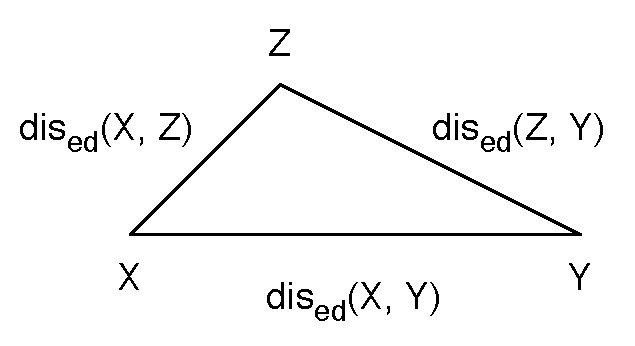
\includegraphics[width=0.4 \textwidth]{fig/triangle01.pdf}}
\quad
\subfigure[]{% b
\label{triIneqb}
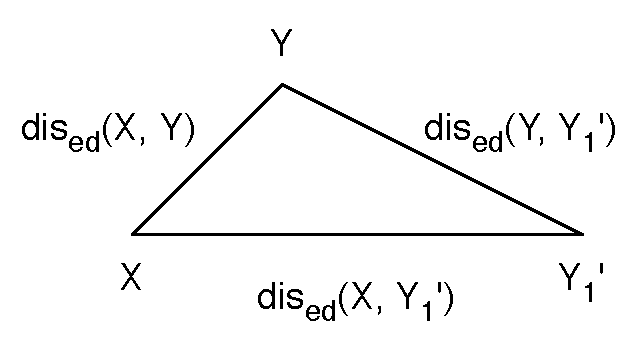
\includegraphics[width=0.4 \textwidth]{fig/triangle02.pdf}}

\caption{Graph Representations for Applying Triangle Inequality}
\label{triIneq}
\end{figure}


\begin{property}[Progressive Bounds for Edit Distance with Unit Penalty Functions]\label{ppt:bound-ed}
Let us consider edit distance with unit penalty functions where the cost for each deletion, insertion, and substitution operation is $1$. Given the edit distance $dis_{ed}(X, Y)$ between two strings $X$ and $Y$, and without the knowledge of the updated string $Y_u'$ after $u$ updates on $Y$, we have 
$$\max\{0, dis_{ed}(X, Y) - 2u\} \leq dis_{ed}(X, Y_u') \leq dis_{ed}(X, Y) + 2u.$$

\end{property}

\begin{proof}
By the definition of edit distance with unit penalty functions and how queries are updated, we have $dis_{ed}(Y, Y'_1)\in \{0,1,2\}$. Let us consider the following triangle inequalities on a triangle with vertices $X$, $Y$, and $Y_1'$, as shown in Figure~\ref{triIneqb}. 
\begin{align}
dis_{ed}(X, Y'_1) &\leq dis_{ed}(X, Y) + dis_{ed}(Y, Y'_1) \label{ineq01}\\
dis_{ed}(X, Y'_1) &\geq |dis_{ed}(X, Y)-dis_{ed}(Y, Y'_1)| \label{ineq02}
\end{align}

From Inequality~\ref{ineq01},~\ref{ineq02}, and the range of $dis_{ed}(Y, Y'_1)$, we have 
% $$\max\{0, dis_{ed}(X, Y) - 2\} \leq dis_{ed}(X, Y'_1) \leq dis_{ed}(X, Y) + 2.$$ 
\begin{align}\label{ineq03}
\max\{0, dis_{ed}(X, Y) - 2\} \leq dis_{ed}(X, Y'_1) \leq dis_{ed}(X, Y) + 2.
\end{align}

More generally, for edit distance after $u$ updates, we can apply Inequality~\ref{ineq03} $u$ times iteratively and get the bounds as stated in the property.
\end{proof}

\begin{property}[Progressive Bounds for Edit Distance with General Penalty Functions]\label{ppt:bound-ed-gen}
Let us consider edit distance with general penalty functions as discussed in Definition~\ref{def:edit-gen}, where the penalties for insertion, deletion and substitution are denoted as $\delta_i$, $\delta_d$, and $\delta_s$, respectively.  Given the edit distance $dis_{ed}(X, Y)$ between two strings $X$ and $Y$, and without the knowledge of the updated string $Y_u'$ after $u$ updates on $Y$, we have 
$$\max\{0, dis_{ed}(X, Y) - u \cdot \max\{\delta_i + \delta_d, \delta_s\} \} \leq dis_{ed}(X, Y_u') \leq dis_{ed}(X, Y) + u \cdot \max\{\delta_i+\delta_d, \delta_s\}\text{.}$$
\end{property}

\begin{proof}
By the definition of edit distance with general penalty functions and how queries are updated, we have $$0 \leq dis_{ed}(Y, Y'_1)\leq \max\{ \delta_i + \delta_d, \delta_s\}\text{.}$$ Let us also apply triangle inequalities on a triangle with vertices $X$, $Y$, and $Y_1'$, as shown in Figure~\ref{triIneqb}. Recalling Inequality~\ref{ineq01} and ~\ref{ineq02} and considering the range of $dis_{ed}(Y, Y'_1)$, we have the following bounds.     
\begin{align}\label{ineq04}
\max\{0, dis_{ed}(X, Y) - \max\{\delta_i + \delta_d, \delta_s\} \} \leq dis_{ed}(X, Y_1') \leq dis_{ed}(X, Y) + \max\{\delta_i+\delta_d, \delta_s\}\text{.}
\end{align}

More generally, for edit distance after $u$ updates, we can apply Inequality~\ref{ineq04} $u$ times iteratively and get the bounds as stated in the property.
\end{proof}


\begin{property}[Progressive Bounds for Edit Similarity with Unit Penalty Functions]\label{ppt:bound-es}
Given the edit similarity $sim_{ed}(X, Y)$ between two strings $X$ and $Y$, and without the knowledge of the updated string $Y_u'$ after $u$ updates on $Y$, we have 
$$sim_{ed}(X, Y)-\frac{2u}{\max\{|X|, |Y|\}} \leq sim_{ed}(X, Y'_u) \leq \min\{1, sim_{ed}(X,Y)+\frac{2u}{\max\{|X|, |Y|\}}\}.$$
\end{property}

\begin{proof}
By the definition of edit similarity and Property~\ref{ppt:bound-ed}, we have 
\begin{align*} 
sim_{ed}(X, Y'_u) &\leq 1 - \frac{\max\{0, dis_{ed}(X, Y) - 2u\}}{\max\{|X|, |Y|\}}\\
&=\min\{1, sim_{ed}(X,Y)+\frac{2u}{\max\{|X|, |Y|\}}\}\\
sim_{ed}(X, Y'_u) &\geq 1 - \frac{dis_{ed}(X, Y) + 2u}{\max\{|X|, |Y|\}}\\
&= sim_{ed}(X, Y)-\frac{2u}{\max\{|X|, |Y|\}}
\end{align*}
\end{proof}

\begin{property}[Progressive Bounds for Edit Similarity with General Penalty Functions]\label{ppt:bound-es-gen}
Given the edit similarity $sim_{ed}(X, Y)$ between two strings $X$ and $Y$, and without the knowledge of the updated string $Y_u'$ after $u$ updates on $Y$, we have 
\begin{align}
sim_{ed}(X, Y'_u) &\geq sim_{ed}(X, Y)-\frac{u\cdot \max\{\delta_i + \delta_d, \delta_s\}}{\max\{\delta_i, \delta_d, \delta_s\} \cdot \max\{|X|, |Y|\}}\\
sim_{ed}(X, Y'_u) &\leq \min\{1, sim_{ed}(X,Y)+\frac{u \cdot \max\{\delta_i + \delta_d, \delta_s\}}{\max\{\delta_i, \delta_d, \delta_s\} \cdot \max\{|X|, |Y|\}}\}.
\end{align}
\end{property}

\begin{proof}
By the definition of edit similarity with general penalty function and Property~\ref{ppt:bound-ed-gen}, we have 
\begin{align*} 
sim_{ed}(X, Y'_u) &\leq 1 - \frac{\max\{0, dis_{ed}(X, Y) - u \cdot \max\{\delta_i + \delta_d, \delta_s\} \}}{\max\{\delta_i, \delta_d, \delta_s\} \cdot \max\{|X|, |Y|\}}\\
&=\min\{1, sim_{ed}(X,Y)+\frac{u \cdot \max\{\delta_i + \delta_d, \delta_s\}}{\max\{\delta_i, \delta_d, \delta_s\} \cdot \max\{|X|, |Y|\}}\}\\
sim_{ed}(X, Y'_u) &\geq 1 - \frac{dis_{ed}(X, Y) + u \cdot \max\{\delta_i + \delta_d, \delta_s\}}{\max\{\delta_i, \delta_d, \delta_s\} \cdot \max\{|X|, |Y|\}}\\
&= sim_{ed}(X, Y)-\frac{u\cdot \max\{\delta_i + \delta_d, \delta_s\}}{\max\{\delta_i, \delta_d, \delta_s\} \cdot \max\{|X|, |Y|\}}
\end{align*}
\end{proof}


\begin{example}[Progressive Bounds for Edit Similarity‎]\label{example:bound-ed}
Let us consider the same strings $X$ and $Y$ as in Example~\ref{example:comp-edit}. If we use unit penalty functions, the edit distance between $X$ and $Y$ is $3$, as shown in Table~\ref{edit02}. The edit similarity is $1-\frac{3}{1*6}=0.50$. Suppose $u=1$, we have $1 \leq dis_{ed}(X, Y_u') \leq 5$ and $0.167 \leq sim_{ed}(X, Y_u') \leq 0.833$. Let us then consider the general penalty functions where $\delta_i = 2, \delta_d = 1$ and $\delta_s = 3$. As shown in Table~\ref{edit01}, the edit distance between $X$ and $Y$ is $8$. Thus, the edit similarity is $1-\frac{8}{3*6} = \frac{5}{9} = 0.56$. Suppose $u=1$, we have $5 \leq dis_{ed}(X, Y_u') \leq 11$ and $0.39 \leq sim_{ed}(X, Y_u') \leq 0.72$.       
\end{example}


\subsection{Cosine Similarity} 
\begin{definition}[Cosine Similarity]\label{def:cosine}
Let us consider the vector representation mentioned in Chapter~\ref{ch:prob-def}. Given two vectors, $\vec{X}$ and $\vec{Y}$, the cosine similarity is defined using a dot product and magnitudes of vectors. 
\begin{align*}   
sim_{cos}(\vec{X}, \vec{Y}) =\frac{\vec{X} \cdot \vec{Y}} {\| \vec{X} \| \| \vec{Y} \|}=\frac{\sum_{i=1}^{|\Sigma|}\vec{X}_{(i)} \times \vec{Y}_{(i)}}{\sqrt{\sum_{i=1}^{|\Sigma|}(\vec{X}_{(i)})^2} \times \sqrt{\sum_{i=1}^{|\Sigma|}(\vec{Y}_{(i)})^2}}
\end{align*}  
where $\vec{X}_{(i)}$ and $\vec{Y}_{(i)}$ are the $i$-th components of vectors $\vec{X}$ and $\vec{Y}$, respectively.  
\end{definition}

\begin{example}[Computation of Cosine Similarity]\label{example:comp-cos}
Given an alphabet $\Sigma=\{e_1, e_2, e_3, e_4, e_5\}$, $X= \{e_3, e_2, e_2, e_1, e_5, e_2, e_1\}$ and $Y = \{e_1, e_2, e_1, e_3, e_5, e_4, e_2, e_3, e_4\}$ are two multisets over $\Sigma$. We can transform $X$ and $Y$ to vectors, that is, $\vec{X} = \{2, 3, 1, 0, 1\}$ and $\vec{Y} = \{2, 2, 2, 2, 1\}$. We have $\vec{X}\cdot \vec{Y} = 13$, $\|\vec{X}\| = \sqrt{15}$ and $\|\vec{Y}\| = \sqrt{17}$. Thus, $sim_{cos}(\vec{X}, \vec{Y}) = \frac{13}{\sqrt{15}*\sqrt{17}} = 0.81$.  
\end{example}

Given the exact cosine similarity, dot product value of two vectors, and statistics on the current query, we can estimate the cosine similarity after a number of updates in constant time. The following property holds for computing the upper and lower bounds for the updated similarity score.

\begin{property} [Progressive Bounds for Cosine Similarity] 
Let us consider two multi-sets $X$ and $Y$ and their corresponding vector representations $\vec{X}$ and $\vec{Y}$. If the exact cosine similarity between $\vec{X}$ and $\vec{Y}$ is $sim_{cos}(\vec{X}, \vec{Y})$, the dot product value is $\vec{X}\cdot \vec{Y}$, and the value of the maximum component of $\vec{X}$ is $h_{\vec{X}}$, then we have the following bounds for cosine similarity after $u$ updates. Note that we use notations $|Y|$, the cardinality of multi-set $Y$, and $\sum_{i=1}^{|\Sigma|}\vec{Y}_{(i)}$ interchangeably.
\begin{align*} 
sim_{cos}(\vec{X}, \vec{Y}_u') &\geq 
\begin{cases}
\frac{1}{\alpha} \cdot (1-\phi)\cdot sim_{cos}(\vec{X}, \vec{Y}) & , \vec{X}\cdot \vec{Y} \neq 0\\
0 & , \vec{X}\cdot \vec{Y} = 0\\
\end{cases}
\end{align*}

\begin{align*}
sim_{cos}(\vec{X}, \vec{Y}_u') &\leq 
\begin{cases}
\frac{1}{\beta} \cdot (1+\phi)\cdot sim_{cos}(\vec{X}, \vec{Y}) & , \vec{X}\cdot \vec{Y} \neq 0\\
\frac{h_{\vec{X}}\cdot u}{\beta \|\vec{X}\|\|\vec{Y}\|} & , \vec{X}\cdot \vec{Y} = 0\\
\end{cases}
\end{align*} 
where $$\alpha=\sqrt{(2u+1)-\frac{u^2+u}{|Y|}}$$ 
$$\beta=\frac{|Y|}{\sqrt{(|Y|-u)^2+u}}$$ 
and 
$$\phi = \frac{h_{\vec{X}}\cdot u}{\vec{X}\cdot \vec{Y}}\hspace{3 mm},\vec{X}\cdot \vec{Y} \neq 0$$ 
\end{property}

\begin{proof}
Let $\vec{Y}_u'$ be the updated vector of $\vec{Y}$ after $u$ updates. Two inequalities used in this proof are as follows.
\begin{align} 
|Y| &\leq \|\vec{Y}\|^2 \leq |Y|^2 \\
\sqrt{\|\vec{Y}\|^2+u-|Y|^2+(|Y|-u)^2} &\leq \|\vec{Y}_u'\| \leq \sqrt{\|\vec{Y}\|^2-u+|Y|^2-(|Y|-u)^2} 
\end{align}

We first prove the lower bound using the above inequalities.

When $\vec{X}\cdot \vec{Y} \neq 0$,
\begin{align*}
sim_{cos}(\vec{X}, \vec{Y_u'}) &= \frac{\vec{X}\cdot \vec{Y_u'}}{\|\vec{X}\|\|\vec{Y_u'}\|} \geq \frac{(\vec{X}\cdot \vec{Y_u'})_{min}}{(\|\vec{X}\|\|\vec{Y_u'}\|)_{max}}\\ 
&= \frac{\vec{X} \cdot \vec{Y}-h_{\vec{X}}\cdot u}{\| \vec{X} \|\cdot \sqrt{\|\vec{Y}\|^2-u+|Y|^2-(|Y|-u)^2}}\\
&= \frac{\vec{X} \cdot \vec{Y}-h_{\vec{X}}\cdot u}{\frac{\vec{X} \cdot \vec{Y}}{sim_{cos}(\vec{X}, \vec{Y})\cdot \|\vec{Y}\|}\cdot\sqrt{\|\vec{Y}\|^2+2u\cdot |Y|-u^2-u}} \\
&= \frac{\|\vec{Y}\|}{\sqrt{\|\vec{Y}\|^2+2u\cdot |Y|-u^2-u}}(1-\frac{h_{\vec{X}}\cdot u}{\vec{X}\cdot \vec{Y}})sim_{cos}(\vec{X}, \vec{Y})\\
&\geq \frac{1}{\sqrt{1+\frac{2u\cdot |Y|-u^2-u}{|Y|}}}(1-\frac{h_{\vec{X}}\cdot u}{\vec{X}\cdot \vec{Y}})sim_{cos}(\vec{X}, \vec{Y})\\
&= \frac{1}{\alpha}(1-\frac{h_{\vec{X}}\cdot u}{\vec{X}\cdot \vec{Y}})sim_{cos}(X, Y)
\end{align*}
where $\alpha=\sqrt{(2u+1)-\frac{u^2+u}{|Y|}}$. \\ \newline
\indent When $\vec{X}\cdot \vec{Y} = 0$,
\begin{align*}
sim_{cos}(\vec{X}, \vec{Y_u'}) &= \frac{\vec{X}\cdot \vec{Y_u'}}{\|\vec{X}\|\|\vec{Y_u'}\|} \geq \frac{(\vec{X}\cdot \vec{Y_u'})_{min}}{(\|\vec{X}\|\|\vec{Y_u'}\|)_{max}} = 0
\end{align*}



The upper bound can be derived similarly.

When $\vec{X}\cdot \vec{Y} \neq 0$,
\begin{align*}
sim_{cos}(\vec{X}, \vec{Y_u'}) &= \frac{\vec{X}\cdot \vec{Y_u'}}{\|\vec{X}\|\|\vec{Y_u'}\|} \leq \frac{(\vec{X}\cdot \vec{Y_u'})_{max}}{(\|\vec{X}\|\|\vec{Y_u'}\|)_{min}} \\
&= \frac{\vec{X} \cdot \vec{Y}+h_{\vec{X}} \cdot u}{\| \vec{X} \| \cdot \sqrt{\|\vec{Y}\|^2+u-|Y|^2+(|Y|-u)^2}}\\
&= \frac{\vec{X} \cdot \vec{Y}+h_{\vec{X}} \cdot u}{\frac{\vec{X} \cdot \vec{Y}}{sim_{cos}(\vec{X}, \vec{Y}) \cdot \|\vec{Y}\|}\cdot \sqrt{\|\vec{Y}\|^2-2u\cdot |Y|+u^2+u}}\\
&= \frac{\|\vec{Y}\|}{\sqrt{\|\vec{Y}\|^2-2u\cdot |Y|+u^2+u}}(1+\frac{h_{\vec{X}}\cdot u}{\vec{X}\cdot \vec{Y}})sim_{cos}(\vec{X}, \vec{Y})\\
&\leq \frac{1}{\sqrt{1+\frac{u^2+u-2u\cdot |Y|}{|Y|^2}}}(1+\frac{h_{\vec{X}}\cdot u}{\vec{X}\cdot \vec{Y}})sim_{cos}(\vec{X}, \vec{Y})\\
&= \frac{1}{\beta}(1+\frac{h_{\vec{X}}\cdot u}{\vec{X}\cdot \vec{Y}})sim_{cos}(\vec{X}, \vec{Y})
\end{align*}
where $\beta=\frac{|Y|}{\sqrt{(|Y|-u)^2+u}}$. \\ \newline
\indent When $\vec{X}\cdot \vec{Y} = 0$,
\begin{align*}
sim_{cos}(\vec{X}, \vec{Y_u'}) &= \frac{\vec{X}\cdot \vec{Y_u'}}{\|\vec{X}\|\|\vec{Y_u'}\|} \leq \frac{(\vec{X}\cdot \vec{Y_u'})_{max}}{(\|\vec{X}\|\|\vec{Y_u'}\|)_{min}} \\
&= \frac{\vec{X} \cdot \vec{Y}+h_{\vec{X}} \cdot u}{\| \vec{X} \| \cdot \sqrt{\|\vec{Y}\|^2+u-|Y|^2+(|Y|-u)^2}}\\
&\leq \frac{h_{\vec{X}} \cdot u}{\| \vec{X} \|\| \vec{Y} \| \sqrt{1+\frac{u^2+u-2u\cdot |Y|}{|Y|^2}}}\\
&= \frac{h_{\vec{X}}\cdot u}{\beta \|\vec{X}\|\|\vec{Y}\|}
\end{align*}

\end{proof}

\begin{example}[Computation of Progressive Bounds for Cosine Similarity] 
Let us consider the same vectors in Example~\ref{example:comp-cos}. We have $\vec{X}\cdot \vec{Y} = 13$, $h_{\vec{X}}=3$, $|Y|=9$ and $sim_{cos}(\vec{X}, \vec{Y}) = 0.81$. Suppose $u=1$, the upper bound of the cosine similarity after an update is $sim_{cos\_up}(\vec{X}, \vec{Y_1'}) = \frac{\sqrt{65}}{9}*(1+\frac{3}{13})*0.81=0.89$ and the corresponding lower bound is $sim_{cos\_lo}(\vec{X}, \vec{Y_1'}) = \frac{3}{5}*(1-\frac{3}{13})*0.81=0.37$.
\end{example}

Our pruning-based method supports the similarity measures defined above and can be further extended to similarity/distance measures, such as hamming distance, overlap similarity and dice similarity, whose progressive bounds can be computed in constant time.


